%REPORT TEMPLATE
%AUTHOR: RUI QU  
%EMAIL: RQU@KTH.SE 

%----------------------------------------------------------------------------------------
%	PACKAGES AND DOCUMENT CONFIGURATIONS
%----------------------------------------------------------------------------------------

\documentclass{article}

%---Basic---
\usepackage{natbib} % Required to change bibliography style to APA
\usepackage{amsmath} % Required for some math elements 
\setlength\parindent{0pt} % Removes all indentation from paragraphs
\usepackage{listings}%Insert code
\usepackage{times} % Uncomment to use the Times New Roman font

%---Table---
\usepackage{multirow}%Table
\usepackage{booktabs}%Table Triple-lines
\usepackage{siunitx} % Provides the \SI{}{} and \si{} command for typesetting SI units

%---Figure---
\usepackage{graphicx} % Required for the inclusion of images
\usepackage{subfigure} % Required for multiple images
\usepackage{float} 

%---Pseudo-code in LaTeX---
\usepackage{algorithm}
\usepackage{algpseudocode}
\usepackage{amsmath}
\renewcommand{\algorithmicrequire}{\textbf{Input:}}  % Use Input in the format of Algorithm
\renewcommand{\algorithmicensure}{\textbf{Output:}} % Use Output in the format of Algorithm

%---Appendix---
\usepackage{appendix}
\newcommand{\upcite}[1]{\textsuperscript{\textsuperscript{\cite{#1}}}} %Upcite

%----------------------------------------------------------------------------------------
%	DOCUMENT INFORMATION
%----------------------------------------------------------------------------------------

\begin{document}

\title{CS-E4950 Computer Vision\\Exercise Round 9}                  
\author{Rui Qu\\rui.qu@aalto.fi}
\maketitle

% If you wish to include an abstract, uncomment the lines below
% \begin{abstract}
% Abstract text
% \end{abstract}

%----------------------------------------------------------------------------------------
%	SECTION 1
%----------------------------------------------------------------------------------------

\section*{Exercise 1 Solution}
\textbf{Schematic Picture of the Network}\footnotemark[1]
\footnotetext[1]{Picture generated via NN-architecture schematics (alexlenail.me/NN-SVG/)}

\begin{figure}[H]
\centering  
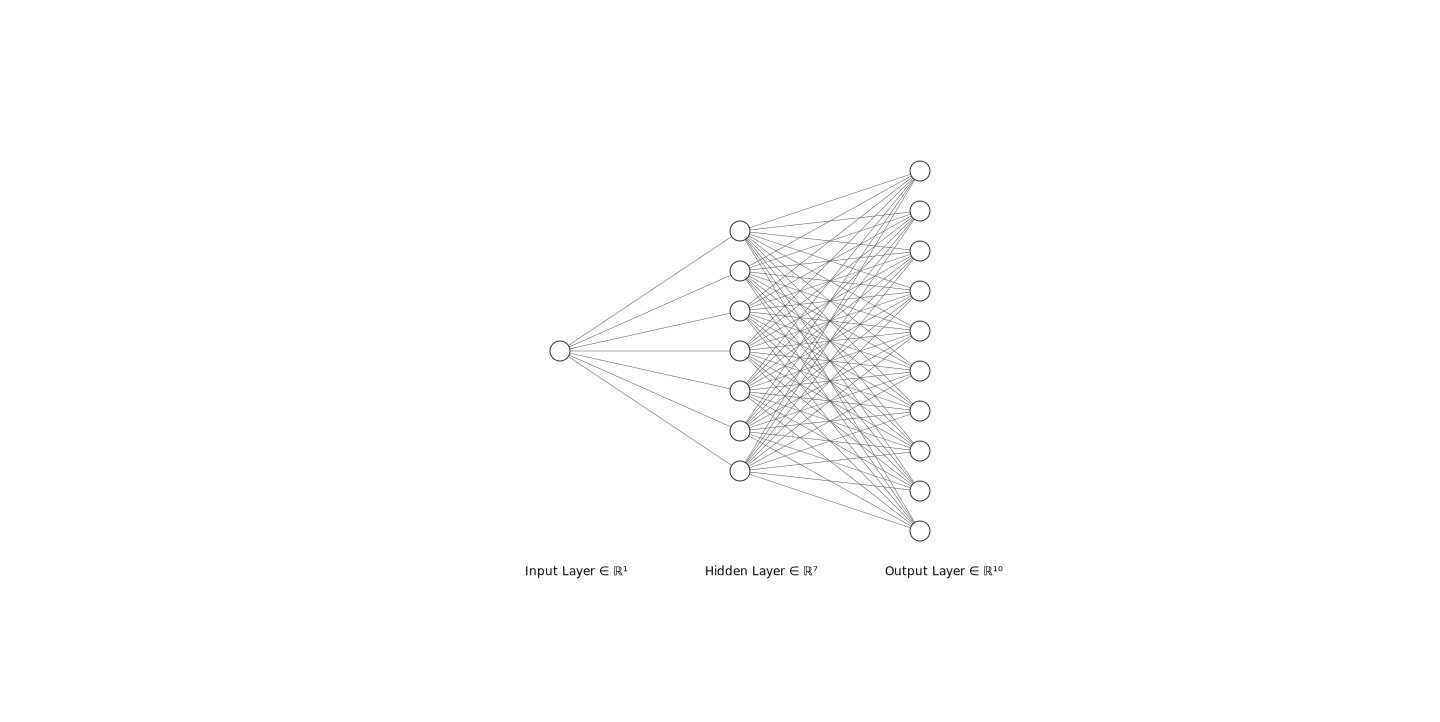
\includegraphics[scale=0.6]{nn.png}
\caption{Fully Connected Neural Network with 1 input}
\label{fig: label}
\end{figure}

\textbf{1.}\\

Given m=1:

\begin{equation}
\begin{aligned}
&E=\frac{1}{m}\sum^m_{j=1}-t_j\cdot log(y_j)\\
&E=-t\cdot log(\mathbf{y})=-t\cdot log(\sigma(\mathbf{W}x))=-t\cdot log\frac{1}{1+e^{-\mathbf{W}x}}\\
\end{aligned}
\end{equation}

Partial derivates of $E$ with respect to $t$ and $x$:

\begin{equation}
\begin{aligned}
\frac{\partial E}{\partial t}&=-log\frac{1}{1+e^{-\mathbf{W}x}}\\
\frac{\partial E}{\partial x}&=-\frac{t}{\sigma(\mathbf{W}x)}\cdot \frac{\partial \sigma(\mathbf{W}x)}{\partial x}\\
&=-t(1+e^{-\mathbf{W}x})\cdot \mathbf{W}\frac{1}{1+e^{-\mathbf{W}x}}(1-\frac{1}{1+e^{-\mathbf{W}x}})\\
&=-t\mathbf{W}\frac{e^{-\mathbf{W}x}}{1+e^{-\mathbf{W}x}}
\end{aligned}
\end{equation}

\textbf{2.}\\

Utilise the chain rule:

\begin{equation}
\begin{aligned}
\frac{\partial E}{\partial z_i^{(2)}}&=\sum^n_{j=1}\frac{\partial E_j}{\partial y_j^{(2)}}\frac{\partial y_j^{(2)}}{\partial z_i^{(2)}}\\
\frac{\partial E_j}{\partial y_j^{(2)}}&=\frac{\partial(-t_j\cdot log y_j)}{\partial z_i^{(2)}}=-\frac{t_j}{y_i}
\label{21}
\end{aligned}
\end{equation}

If $i\neq j$:
\begin{equation}
\begin{aligned}
\frac{\partial y_j^{(2)}}{\partial z_i^{(2)}}=\frac{\partial \sigma(z_j^{(2)})}{\partial z_i^{(2)}}=-y_iy_j
\label{22}
\end{aligned}
\end{equation}

If $i=j$:
\begin{equation}
\begin{aligned}
\frac{\partial y_j^{(2)}}{\partial z_i^{(2)}}=\frac{\partial \sigma(z_i^{(2)})}{\partial z_i^{(2)}}=y_i(1-y_i)
\label{23}
\end{aligned}
\end{equation}

Derived from Equation (\ref{21}) (\ref{22}) (\ref{23}) and $\sum t_j=1$:

\begin{equation}
\begin{aligned}
\frac{\partial E}{\partial z_i^{(2)}}&=\sum^n_{j=1}\frac{\partial E_j}{\partial y_j^{(2)}}\frac{\partial y_j^{(2)}}{\partial z_i^{(2)}}\\ =&\sum_{i\neq j}\frac{\partial E_j}{\partial y_j^{(2)}}\frac{\partial y_j^{(2)}}{\partial z_i^{(2)}}+\sum_{i=j}\frac{\partial E_j}{\partial y_j^{(2)}}\frac{\partial y_j^{(2)}}{\partial z_i^{(2)}}\\
=&\sum_{i\neq j}[-\frac{t_j}{y_i}(-y_iy_j)] -\frac{t_j}{y_i}y_i(1-y_i)\\
=&\sum_{i\neq j}[(t_jy_i)] +t_iy_i-t_i\\
=&y_i-t_i
\end{aligned}
\end{equation}

Hence:

\begin{equation}
\begin{aligned}
\frac{\partial E}{\partial \mathbf{z}^{(2)}}=(\mathbf{y}^{(2)}-\mathbf{t})^\top
\end{aligned}
\end{equation}

\textbf{3.}\\

\begin{equation}
\begin{aligned}
\frac{\partial E}{\partial \mathbf{z}^{(2)}}&=(\mathbf{y}^{(2)}-\mathbf{t})^\top\\
\frac{\partial E}{\partial \mathbf{y}^{(1)}}&=\frac {\partial E}{\partial z^(2)}\cdot \frac {\partial z^(2)}{\partial y^(1)}=(\mathbf{y}^{(2)}-\mathbf{t})^\top\cdot\mathbf{W}^{(2)}
\end{aligned}
\end{equation}

\textbf{4.}\\
\begin{equation}
\begin{aligned}
\frac{\partial E}{\partial W_{uv}^{(2)}}&=\frac{\partial E}{\partial \mathbf{z}^{(2)}}\frac{\partial \mathbf{z}^{(2)}}{\partial W_{uv}^{(2)}}\\
&=(\frac{\partial E}{\partial \mathbf{z}^{(2)}})_uy_v^{(1)}\\
&=(y_u^{(2)}-t_u)y_v^{(1)} \\
i.e. \frac{\partial E}{\partial \mathbf W^{(2)}}&=[(\mathbf y^{(2)}-\mathbf t)\mathbf y^{(1)} ]^\top
\end{aligned}
\end{equation}


\textbf{5.}\\
\begin{equation}
\begin{aligned}
\frac{\partial \mathbf y^{(1)}}{\partial \mathbf z^{(1)}}&=\mathbf y^{(1)}(1-\mathbf y^{(1)})=diag(\mathbf y^{(1)}*(1-\mathbf y^{(1)}))\\
\frac{\partial \sigma( z)}{\partial z}&=\frac{-(-1)e^{-z}}{(1+e^{- z})^2}\\
&=\frac{1}{1+e^{- z}}\cdot \frac{e^{-z}}{1+e^{-z}}\\
&=\sigma(z)(1-\sigma(z))
\end{aligned}
\end{equation}

\textbf{6.}\\

\begin{equation}
\begin{aligned}
\frac{\partial E}{\partial \mathbf{z}^{(1)}}&=\frac{\partial E}{\partial \mathbf{y}^{(1)}}\frac{\partial \mathbf y^{(1)}}{\partial \mathbf{z}^{(1)}}\\
&=(\mathbf y^{(2)}-t)^\top \mathbf W^{(2)}diag(\mathbf y^{(1)})*(1-\mathbf y^{(1)})
\end{aligned}
\end{equation}


\textbf{7.}\\
\begin{equation}
\begin{aligned}
\frac{\partial E}{\partial W_{uv}^{(1)}}&=\frac{\partial E}{\partial \mathbf{z}^{(1)}}\frac{\partial \mathbf{z}^{(1)}}{\partial W_{uv}^{(1)}}\\
&=\frac{\partial E}{\partial z_u^{(1)}} \frac{\partial \mathbf z_u}{\partial w_{uv}^{(1)}} \\
&=\frac{\partial E}{\partial z_u^{(1)}} \frac{\partial(\sum_i w_{ui}x_i)}{\partial w_{uv}}\\
&=\frac{\partial E}{\partial z_u^{(1)}}x_v\\
i.e.\frac{\partial E}{\partial \mathbf W^{(1)}}&=(\frac{\partial E}{\partial \mathbf z^{(1)}})^\top\mathbf x^\top
\end{aligned}
\end{equation}





\end{document}